\section{Modèle avec composante IT, WR et CR (FIRE-IT-WR-CR)}
\subsection{Question 2.3.1}
Les lignes suivantes seront ajoutées à la fin de l'algorithme interact-with. Le fournisseur choisit la meilleure note parmi celles que le consommateur a enregistré. Il gardera donc toujours une note par interaction avec un consommateur différent mais il peut choisir la meilleure parmi ces interactions.
\begin{algorithm}[H]
\caption{Store certified reputation}

\begin{algorithmic}
\STATE allRatings $\leftarrow$ get-rates-for (provider)
\STATE bestRate $\leftarrow$ max(allRatings)
\STATE provider.receivedRatings $\leftarrow$ provider.receivedRatings $\cup$ bestRate

\end{algorithmic}
\end{algorithm}

Donc \texttt{get-rates(CR, p)} renvoie la liste \texttt{receivedRatings} (de taille H au maximum) du fournisseur p.

\subsection{Question 2.3.2}
Nous avons modifié le code afin que le système prenne un nouveau paramètre en compte : la différence de distance lorsqu'on a une note venant d'un autre consommateur (WR ou CR) car il y a des chances que ce dernier soit plus proche du fournisseur. Il faut donc ajuster la performance attendue en fonction de cette différence. Le calcul de celle-ci est décrit dans la partie \hyperref[sec:hypotheses]{Hypothèses}. Cette modification a été faite dès l'implémentation du composant WR.

\subsection{Question 2.3.3}
\begin{figure}[H]
   \begin{minipage}{0.48\textwidth}
     \centering
     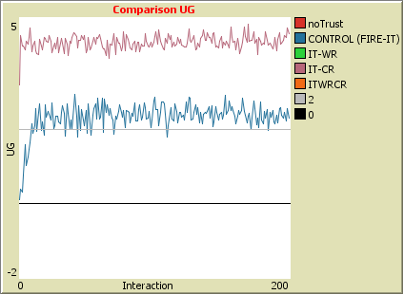
\includegraphics[width=.7\linewidth]{images/ITvsITCR.png}
     \caption{Reproduction figure 10 (ITWR - ITCR)}\label{Fig:Data1}
   \end{minipage}\hfill
   \begin{minipage}{0.48\textwidth}
     \centering
     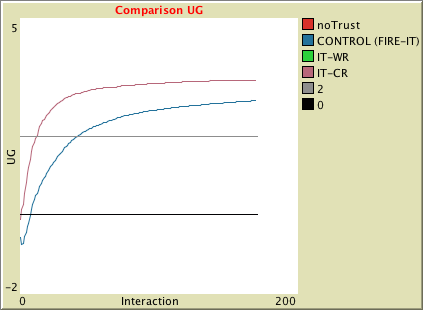
\includegraphics[width=.7\linewidth]{images/ITvsITCR2.png}
     \caption{IT-ITCR sans vider les UGs}\label{Fig:Data2}
   \end{minipage}
\end{figure}

\begin{figure}[H]
\centering
\captionsetup{justification=centering}
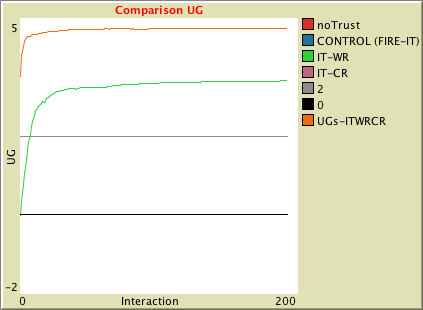
\includegraphics[width=0.4\linewidth]{images/ITWRvsITWRCR.png}
\caption{Reproduction figure 11 (ITWR - ITWRCR)}
\label{fig:fig11}
\end{figure}

Afin de rendre le résultat plus lisible, nous avons gardé les listes des UGs sans les vider pour la reproduction de la figure 11.
Nous remarquons que la présence du composant CR donne une UG quasiment égale à celle que nous apportait le composant WR tout en étant beaucoup plus rapide. La recherche de témoins prenait beaucoup plus temps à s'exécuter, ce qui est compréhensible étant donné le grand nombre d'agents. Le modèle ITCR est aussi beaucoup plus performant dès les premières interactions, ce qui est logique car il y a 100 fournisseurs pour 500 consommateurs. Un fournisseur a plus de chances d'effectuer sa première interaction plus vite qu'un consommateur.
Sur la figure 11, nous remarquons que le modèle ITWRCR converge plus vite que ITWR. Nous supposons que, grâce à une collecte rapide des informations (via CR), les agents connaissent plus vite leur environnement et se mettent en mode 'exploitation' plus rapidement.

\subsection{Question 2.3.4}
\begin{figure}[H]
\centering
\captionsetup{justification=centering}
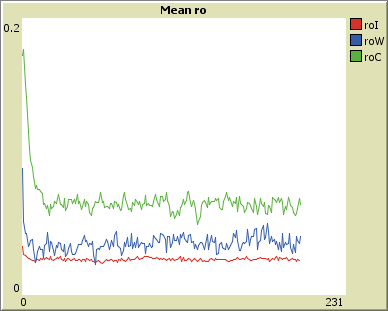
\includegraphics[width=0.8\textwidth]{images/ROs.png}
\label{fig:ROs}
\end{figure}
Nous remarquons que les trois courbes diminuent rapidement. Cependant les fiabilités de IT restent très basses et stables pendant toute la simulation.
D'autre part, la courbe des fiabilité de la composante CR reste au dessus de celle de WR qui est, elle même, au dessus de celle de IT. L'explication pour ce phénomène est le poids des composantes : $W_I$=2, $W_W$=1 et $W_C$=0.5.
Nous remarquons que l'évolution des courbes reflète symétriquement celle des courbes des UGs. Il faut rappeler que les choix entre exploration et exploitation étaient les facteurs principaux des apparences de ces courbes. En effet, les probabilités de choisir une action ou une autre sont à peu près égales au début ($p_{a1}$=$p_{a2}$=0.5). Puis la probabilité de choisir l'exploitation plutôt que l'exploration augmente. Cette évolution correspond à la quantité d'informations qu'un agent possède sur son monde. Nous pouvons donc supposer que la tendance à exploiter ces informations est à l'origine de la diminution des valeurs de fiabilité.